\documentclass{beamer}
\usepackage[utf8]{inputenc}

\usetheme{Madrid}
\usecolortheme{default}
\usepackage{amsmath,amssymb,amsfonts,amsthm}
\usepackage{txfonts}
\usepackage{tkz-euclide}
\usepackage{listings}
\usepackage{adjustbox}
\usepackage{array}
\usepackage{tabularx}
\usepackage{gvv}
\usepackage{lmodern}
\usepackage{circuitikz}
\usepackage{tikz}
\usepackage{graphicx}

\setbeamertemplate{page number in head/foot}[totalframenumber]

\usepackage{tcolorbox}
\tcbuselibrary{minted,breakable,xparse,skins}



\definecolor{bg}{gray}{0.95}
\DeclareTCBListing{mintedbox}{O{}m!O{}}{%
	breakable=true,
	listing engine=minted,
	listing only,
	minted language=#2,
	minted style=default,
	minted options={%
		linenos,
		gobble=0,
		breaklines=true,
		breakafter=,,
		fontsize=\small,
		numbersep=8pt,
		#1},
	boxsep=0pt,
	left skip=0pt,
	right skip=0pt,
	left=25pt,
	right=0pt,
	top=3pt,
	bottom=3pt,
	arc=5pt,
	leftrule=0pt,
	rightrule=0pt,
	bottomrule=2pt,
	toprule=2pt,
	colback=bg,
	colframe=orange!70,
	enhanced,
	overlay={%
		\begin{tcbclipinterior}
			\fill[orange!20!white] (frame.south west) rectangle ([xshift=20pt]frame.north west);
	\end{tcbclipinterior}},
	#3,
}
\lstset{
	language=C,
	basicstyle=\ttfamily\small,
	keywordstyle=\color{blue},
	stringstyle=\color{orange},
	commentstyle=\color{green!60!black},
	numbers=left,
	numberstyle=\tiny\color{gray},
	breaklines=true,
	showstringspaces=false,
}
%------------------------------------------------------------
%This block of code defines the information to appear in the
%Title page
\title %optional
{4.3.32}

%\subtitle{A short story}

\author % (optional)
{Nipun Dasari - EE25BTECH11042}



\begin{document}
	
	\frame{\titlepage}
	\begin{frame}{Question}
		Find the slope of a line which cuts off intercepts of equal length on the axes is. Solve using matrices. \\
	\end{frame}
	
	
	\begin{frame}{Theoretical Solution}
	Consider normal form of a line:
	\begin{align}
		\vec{n}^T\vec{x} = c, \text{where } \vec{n} = \begin{myvec}{n_1\\ n_2}\end{myvec}
	\end{align}
Consider normal form of a line:
\begin{align}
	\vec{n}^\top\vec{x} = 1
\end{align}
Given that equal intercepts are cut off we get 2 cases:\\
On substituting the intercepts in place of $\vec{x}$: \\
\textbf{Case 1: The intercepts are equal \brak{b = a}}
\begin{align}
	\implies  \vec{n}^\top\begin{myvec}{a \\ 0} \end{myvec} = 1  \label{0.2}\\
	\implies \vec{n}^\top\begin{myvec}{0 \\ a} \end{myvec} = 1  \label{0.3} \\
\end{align}

from \eqref{0.2} and from \eqref{0.3}
\begin{align}
	\vec{n}^\top\begin{myvec}{a & 0 \\ 0 & a} \end{myvec} = \begin{myvec}{1 & 1} \end{myvec} \\
	\implies a\vec{n}^\top\begin{myvec}{1 & 0 \\ 0 & 1}\end{myvec} = \begin{myvec}{1 & 1} \end{myvec}\\
	\implies a\vec{n}^\top\vec{I} = \begin{myvec}{1 & 1} \end{myvec}
	\implies a\vec{n}^\top = \begin{myvec}{1 & 1} \end{myvec}
	\implies \vec{n} = \frac{1}{a}\begin{myvec}{1 \\ 1} \end{myvec}
\end{align}
Thus, direction vector $\vec{n} = \begin{myvec}{1 \\ 1}\end{myvec}$
		
	\end{frame}
		\begin{frame}{Theoretical Solution}
			\textbf{Case 2: The intercepts are negatives of each other \brak{-b = a}}
		\begin{align}
			\implies  \vec{n}^\top\begin{myvec}{a \\ 0} \end{myvec} = 1 \label{0.5}\\
			\implies \vec{n}^\top\begin{myvec}{0 \\ -a} \end{myvec} =1\label{0.6} \\
		\end{align}
		By \eqref{0.5}, \eqref{0.6}:
		\begin{align}
			\vec{n}^\top\begin{myvec}{a & 0 \\ 0 & -a} \end{myvec} = \begin{myvec}{1 & 1} \end{myvec} \\
			\implies a\vec{n}^\top\begin{myvec}{1 & 0 \\ 0 & -1}\end{myvec} = \begin{myvec}{1 & 1} \end{myvec}
		\end{align}
		Let $\vec{A} = \begin{myvec}{1 & 0 \\ 0 & -1}\end{myvec}$\\
		For this matrix $\vec{A} = \vec{A}^{-1}$
		\begin{align}
			\implies a\vec{n}^\top = \begin{myvec}{1 & 1}\vec{A}^{-1} \end{myvec}
			\implies a\vec{n}^\top = \begin{myvec}{1 & 1}\vec{A}^{-1} \end{myvec}
			\implies \vec{n} = \frac{1}{a}\begin{myvec}{1 \\ -1} \end{myvec}
		\end{align}
		Thus, direction vector $\vec{n} = \begin{myvec}{1 \\ -1}\end{myvec}$
		The direction vector is given \brak{\text{in general}} by:
		\begin{align}
			\vec{m} = 	\begin{myvec}{1\\ m}\end{myvec} \text{  where $m$ is slope of given line }
		\end{align}		
		On comparing with the obtained direction vectors
		\begin{align}
			\therefore m = \pm1
		\end{align}	
		\end{frame}
	
	\begin{frame}[fragile]
		\frametitle{C Code}
		
		\begin{lstlisting}
			#include <stdio.h>
			void calculate_slopes(double intercept_a, double* output_slopes) {
				// A line requires non-zero intercepts. If a is zero, we can't calculate a slope.
				if (intercept_a == 0.0) {
					output_slopes[0] = 0.0; // Or some error value like NAN
					output_slopes[1] = 0.0;
					return;
				}
				double slope1 = intercept_a / (-intercept_a);
				double slope2 = (-intercept_a) / (-intercept_a);
				// Fill the output array with the two calculated slopes
				output_slopes[0] = slope1;
				output_slopes[1] = slope2;
			}
		\end{lstlisting}
	\end{frame}
	
	\begin{frame}[fragile]
		\frametitle{Python Code using shared output}
		\begin{lstlisting}
			import ctypes
			import numpy as np
			import matplotlib.pyplot as plt
			
			# --- Step 1: Load the shared library ---
			
			lib = ctypes.CDLL('./4.3.32.so')
			
			
			# --- Step 2: Define the C function signature ---
			calculate_slopes_func = lib.calculate_slopes
			calculate_slopes_func.argtypes = [
			ctypes.c_double,
			np.ctypeslib.ndpointer(dtype=np.double, ndim=1, flags='C_CONTIGUOUS')
			]
			calculate_slopes_func.restype = None
		\end{lstlisting}
	\end{frame}
	\begin{frame}[fragile]
		\frametitle{Python Code using shared output}
		\begin{lstlisting}		
		# --- Step 3: Prepare data and call the C function ---
		intercept_a = 4.0
		output_slopes = np.zeros(2, dtype=np.double)
		calculate_slopes_func(intercept_a, output_slopes)
		
		print(f"C function called with intercept a = {intercept_a}")
		print(f"Calculated slopes returned: {output_slopes[0]} and {output_slopes[1]}")
		
		# --- Step 4: Plot the results with highlighted axes ---
		
		fig, ax = plt.subplots(figsize=(8, 8))
		
		# Define x values for plotting the lines
		x = np.linspace(-6, 6, 400)
		
		\end{lstlisting}
	\end{frame}
	\begin{frame}[fragile]
		\frametitle{Python Code using shared output}
		\begin{lstlisting}
		# --- Line 1 (Slope = -1) ---
		slope1 = output_slopes[0]
		y_intercept1 = intercept_a
		y1 = slope1 * x + y_intercept1
		ax.plot(x, y1, 'r-', label=f'Line 1: y = {slope1}x + {y_intercept1:.0f}')
		ax.plot([intercept_a, 0], [0, y_intercept1], 'ro', markersize=8)
		
		# --- Line 2 (Slope = 1) ---
		slope2 = output_slopes[1]
		y_intercept2 = -intercept_a
		y2 = slope2 * x + y_intercept2
		ax.plot(x, y2, 'b-', label=f'Line 2: y = {slope2}x - {y_intercept2:.0f}')
		ax.plot([intercept_a, 0], [0, y_intercept2], 'bo', markersize=8)
		\end{lstlisting}
	\end{frame}
	\begin{frame}[fragile]
		\frametitle{Python Code using shared output}
		\begin{lstlisting}
			# --- Highlighting the Coordinate Axes ---
			# Remove the default box-like plot frame (spines)
			ax.spines['right'].set_color('none')
			ax.spines['top'].set_color('none')
			
			# Move the bottom and left spines to the center (0,0)
			ax.spines['bottom'].set_position('zero')
			ax.spines['left'].set_position('zero')
			
			# Make the new axes bold
			ax.spines['bottom'].set_linewidth(1.5)
			ax.spines['left'].set_linewidth(1.5)
		\end{lstlisting}
	\end{frame}
	
	\begin{frame}[fragile]
		\frametitle{Python Code using shared output}
		\begin{lstlisting}
		# Add arrows to the end of the new axes
		ax.plot(1, 0, ">k", transform=ax.get_yaxis_transform(), clip_on=False)
		ax.plot(0, 1, "^k", transform=ax.get_xaxis_transform(), clip_on=False)
		# --- End of Highlighting Section ---
		
		# --- Plot Styling ---
		ax.set_title('Lines with Intercepts of Equal Length', fontsize=16)
		# Add axis labels at the end of the arrows
		ax.set_xlabel('X-axis', fontsize=12, loc='right')
		ax.set_ylabel('Y-axis', fontsize=12, loc='top', rotation=0)
		
	
		\end{lstlisting}
	\end{frame}
	
	\begin{frame}[fragile]
		\frametitle{Python Code using shared outut}
		\begin{lstlisting}
			ax.set_aspect('equal', adjustable='box')
		ax.grid(True, linestyle=':')
		ax.legend()
		ax.set_xlim(-6, 6)
		ax.set_ylim(-6, 6)
		
		plt.savefig('slope_plot_highlighted.png')
		
		plt.show()
		\end{lstlisting}
	\end{frame}
	
	\begin{frame}{Plot by python using shared output from c}
		\begin{center}
			\begin{figure}[H]
				\centering
				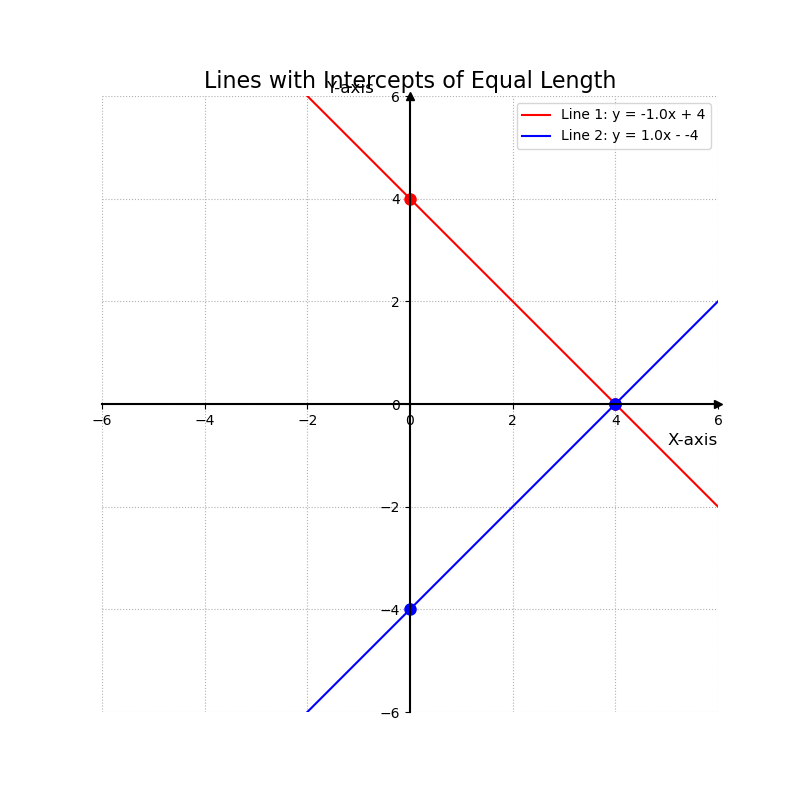
\includegraphics[width = 0.6\columnwidth]{figs/Figure_1.png}
				\caption*{}
				\label{}
			\end{figure}
		\end{center}
	\end{frame}
	
	
\end{document}